% Options for packages loaded elsewhere
\PassOptionsToPackage{unicode}{hyperref}
\PassOptionsToPackage{hyphens}{url}
%
\documentclass[
]{article}
\usepackage{lmodern}
\usepackage{amssymb,amsmath}
\usepackage{ifxetex,ifluatex}
\ifnum 0\ifxetex 1\fi\ifluatex 1\fi=0 % if pdftex
  \usepackage[T1]{fontenc}
  \usepackage[utf8]{inputenc}
  \usepackage{textcomp} % provide euro and other symbols
\else % if luatex or xetex
  \usepackage{unicode-math}
  \defaultfontfeatures{Scale=MatchLowercase}
  \defaultfontfeatures[\rmfamily]{Ligatures=TeX,Scale=1}
\fi
% Use upquote if available, for straight quotes in verbatim environments
\IfFileExists{upquote.sty}{\usepackage{upquote}}{}
\IfFileExists{microtype.sty}{% use microtype if available
  \usepackage[]{microtype}
  \UseMicrotypeSet[protrusion]{basicmath} % disable protrusion for tt fonts
}{}
\makeatletter
\@ifundefined{KOMAClassName}{% if non-KOMA class
  \IfFileExists{parskip.sty}{%
    \usepackage{parskip}
  }{% else
    \setlength{\parindent}{0pt}
    \setlength{\parskip}{6pt plus 2pt minus 1pt}}
}{% if KOMA class
  \KOMAoptions{parskip=half}}
\makeatother
\usepackage{xcolor}
\IfFileExists{xurl.sty}{\usepackage{xurl}}{} % add URL line breaks if available
\IfFileExists{bookmark.sty}{\usepackage{bookmark}}{\usepackage{hyperref}}
\hypersetup{
  pdftitle={Microbiota},
  pdfauthor={Marco Chiapello},
  hidelinks,
  pdfcreator={LaTeX via pandoc}}
\urlstyle{same} % disable monospaced font for URLs
\usepackage[margin=1in]{geometry}
\usepackage{graphicx}
\makeatletter
\def\maxwidth{\ifdim\Gin@nat@width>\linewidth\linewidth\else\Gin@nat@width\fi}
\def\maxheight{\ifdim\Gin@nat@height>\textheight\textheight\else\Gin@nat@height\fi}
\makeatother
% Scale images if necessary, so that they will not overflow the page
% margins by default, and it is still possible to overwrite the defaults
% using explicit options in \includegraphics[width, height, ...]{}
\setkeys{Gin}{width=\maxwidth,height=\maxheight,keepaspectratio}
% Set default figure placement to htbp
\makeatletter
\def\fps@figure{htbp}
\makeatother
\setlength{\emergencystretch}{3em} % prevent overfull lines
\providecommand{\tightlist}{%
  \setlength{\itemsep}{0pt}\setlength{\parskip}{0pt}}
\setcounter{secnumdepth}{-\maxdimen} % remove section numbering
\ifluatex
  \usepackage{selnolig}  % disable illegal ligatures
\fi

\title{Microbiota}
\usepackage{etoolbox}
\makeatletter
\providecommand{\subtitle}[1]{% add subtitle to \maketitle
  \apptocmd{\@title}{\par {\large #1 \par}}{}{}
}
\makeatother
\subtitle{Lesson 1}
\author{Marco Chiapello}
\date{???}

\begin{document}
\maketitle

class: title-slide

\hypertarget{font170microbioma-e-microbiota}{%
\section{.font170{[}MICROBIOMA E
MICROBIOTA{]}}\label{font170microbioma-e-microbiota}}

.marco{[} Marco Chiapello 2020-09-22{]}

.marco{[} .font90{[}{[}\textless svg
style="height:0.8em;top:.04em;position:relative;fill:steelblue;"
viewBox="0 0 512 512"\textgreater\textless path d="M459.37 151.716c.325
4.548.325 9.097.325 13.645 0 138.72-105.583 298.558-298.558
298.558-59.452 0-114.68-17.219-161.137-47.106 8.447.974 16.568 1.299
25.34 1.299 49.055 0 94.213-16.568
130.274-44.832-46.132-.975-84.792-31.188-98.112-72.772 6.498.974 12.995
1.624 19.818 1.624 9.421 0 18.843-1.3
27.614-3.573-48.081-9.747-84.143-51.98-84.143-102.985v-1.299c13.969
7.797 30.214 12.67 47.431
13.319-28.264-18.843-46.781-51.005-46.781-87.391 0-19.492 5.197-37.36
14.294-52.954 51.655 63.675 129.3 105.258 216.365
109.807-1.624-7.797-2.599-15.918-2.599-24.04 0-57.828 46.782-104.934
104.934-104.934 30.213 0 57.502 12.67 76.67 33.137 23.715-4.548
46.456-13.32 66.599-25.34-7.798 24.366-24.366 44.833-46.132 57.827
21.117-2.273 41.584-8.122 60.426-16.243-14.292 20.791-32.161
39.308-52.628
54.253z"/\textgreater\textless/svg\textgreater{]}(https://twitter.com/marpello1980)
@marpello1980 - {[}\textless svg
style="height:0.8em;top:.04em;position:relative;fill:steelblue;"
viewBox="0 0 512 512"\textgreater\textless path d="M502.3 190.8c3.9-3.1
9.7-.2 9.7 4.7V400c0 26.5-21.5 48-48 48H48c-26.5
0-48-21.5-48-48V195.6c0-5 5.7-7.8 9.7-4.7 22.4 17.4 52.1 39.5 154.1
113.6 21.1 15.4 56.7 47.8 92.2 47.6 35.7.3 72-32.8 92.3-47.6 102-74.1
131.6-96.3 154-113.7zM256 320c23.2.4 56.6-29.2 73.4-41.4 132.7-96.3
142.8-104.7 173.4-128.7 5.8-4.5 9.2-11.5
9.2-18.9v-19c0-26.5-21.5-48-48-48H48C21.5 64 0 85.5 0 112v19c0 7.4 3.4
14.3 9.2 18.9 30.6 23.9 40.7 32.4 173.4 128.7 16.8 12.2 50.2 41.8 73.4
41.4z"/\textgreater\textless/svg\textgreater{]}(mailto:chiapello.m@gmail.com)
chiapello.m@gmail.com - \textless svg
style="height:0.8em;top:.04em;position:relative;fill:steelblue;"
viewBox="0 0 448 512"\textgreater\textless path d="M424.7 299.8c2.9-14
4.7-28.9 4.7-43.8 0-113.5-91.9-205.3-205.3-205.3-14.9 0-29.7 1.7-43.8
4.7C161.3 40.7 137.7 32 112 32 50.2 32 0 82.2 0 144c0 25.7 8.7 49.3 23.3
68.2-2.9 14-4.7 28.9-4.7 43.8 0 113.5 91.9 205.3 205.3 205.3 14.9 0
29.7-1.7 43.8-4.7 19 14.6 42.6 23.3 68.2 23.3 61.8 0 112-50.2 112-112
.1-25.6-8.6-49.2-23.2-68.1zm-194.6 91.5c-65.6 0-120.5-29.2-120.5-65 0-16
9-30.6 29.5-30.6 31.2 0 34.1 44.9 88.1 44.9 25.7 0 42.3-11.4 42.3-26.3
0-18.7-16-21.6-42-28-62.5-15.4-117.8-22-117.8-87.2 0-59.2 58.6-81.1
109.1-81.1 55.1 0 110.8 21.9 110.8 55.4 0 16.9-11.4 31.8-30.3 31.8-28.3
0-29.2-33.5-75-33.5-25.7 0-42 7-42 22.5 0 19.8 20.8 21.8 69.1 33 41.4
9.3 90.7 26.8 90.7 77.6 0 59.1-57.1 86.5-112
86.5z"/\textgreater\textless/svg\textgreater{} marpello{]}{]}

???

.n30{[}

\begin{itemize}
\tightlist
\item
  Sarò uno dei vostri docenti per il corso ``Interazioni tra piante,
  microrganismi e ambiente'' {]} --- layout: true class: clear
\end{itemize}

\begin{center}\rule{0.5\linewidth}{0.5pt}\end{center}

.font180{[}.bold{[}Agenda{]}{]}

.h35{[} - .font140{[}Introduzione{]}

\begin{itemize}
\item
  .font120{[}Il microbiota umano{]}
\item
  .font140{[}Il microbiota delle piante{]}

  \begin{itemize}
  \item
    .font120{[}Da chi è composto{]}
  \item
    .font120{[}Che funzioni ha{]}
  \item
    .font120{[}Come prende forma{]} {]}
  \end{itemize}
\end{itemize}

???

\begin{itemize}
\item ~
  \hypertarget{nintro-spiegazione-dei-concetti-generali-e-dei-termini}{%
  \subsection{\texorpdfstring{.n{[}\textbf{Intro}: spiegazione dei
  concetti generali e dei
  termini{]}}{.n{[}Intro: spiegazione dei concetti generali e dei termini{]}}}\label{nintro-spiegazione-dei-concetti-generali-e-dei-termini}}
\end{itemize}

.pull-left{[}.center{[}.font180{[}.bold{[}microBIOTA{]}{]}{]}

\begin{center}\includegraphics[width=400px]{images/microbiota} \end{center}

\textgreater{} .font80{[}si riferisce a una popolazione di microrganismi
che colonizza un determinato luogo{]}

{]}

.pull-right{[}.center{[}.font180{[}.bold{[}microBIOMA{]}{]}{]}

\begin{center}\includegraphics[width=400px]{images/microbioma} \end{center}

\begin{quote}
.font80{[}indica la totalità del patrimonio genetico posseduto dal
microbiota, cioè i geni che quest'ultimo è in grado di esprimere{]}
\end{quote}

{]}

???

\begin{itemize}
\item
  .n{[}si riferisce a una popolazione di microrganismi che colonizza un
  determinato luogo{]}
\item
  .n{[}batteri, funghi, protozoi, elminti, neamtodi, virus, {]}
\item
  .n{[}indica la totalità del patrimonio genetico posseduto dal
  microbiota, cioè i geni che quest'ultimo è in grado di esprimere{]}
\item
  .n{[}la differenza che passa tra i due termini è la stessa che esiste
  tra popolazione umana e genoma umano{]}
\end{itemize}

\begin{center}\rule{0.5\linewidth}{0.5pt}\end{center}

.pull-left{[}.center{[}.font180{[}.bold{[}microBIOTA{]}{]}{]}{]}

.pull-right{[}.center{[}.font180{[}.bold{[}microBIOMA{]}{]}{]}{]}

\begin{center}\includegraphics[width=550px]{images/microPublications} \end{center}

Il \textbf{progetto microbioma umano} è una iniziativa dei National
Institutes of Health statunitensi con il fine di \textbf{identificare e
caratterizzare i microrganismi ed il loro rapporto con lo stato di
salute e di malattia dell'uomo}.

\begin{center}\includegraphics[width=700px]{images/microNubers} \end{center}

???

\begin{itemize}
\item
  .n{[}\textbf{RAPPORTO} cellule microbiche e cellule umane{]}
\item
  .n{[}Il numero totale di cellule microbiche presenti in un organismo
  umano può superare di dieci volte il numero di cellule dell'organismo
  stesso{]}
\item
  .n{[}i geni di origine microbica possono superare di cento volte il
  numero di geni presenti nel genoma umano (composto da circa 20.000
  geni).{]}
\end{itemize}

\begin{center}\rule{0.5\linewidth}{0.5pt}\end{center}

.content-box-grey{[}.font180{[}.fontW7{[}L'essere umano va concepito
come composto da cellule umane e microbiche{]}{]}{]}

???

\begin{itemize}
\item
  .n{[}Visto l'alto numero di cellule microbiche e della quantità del
  loro materiale genetico{]}
\item
  .n{[}L'essere umano va concepito come composto da cellule umane e
  microbiche{]}
\item
  .n{[}MA \textbf{quali} sono i micro-organismi{]}
\end{itemize}

.center{[}Spatial human microbiota{]}

\begin{center}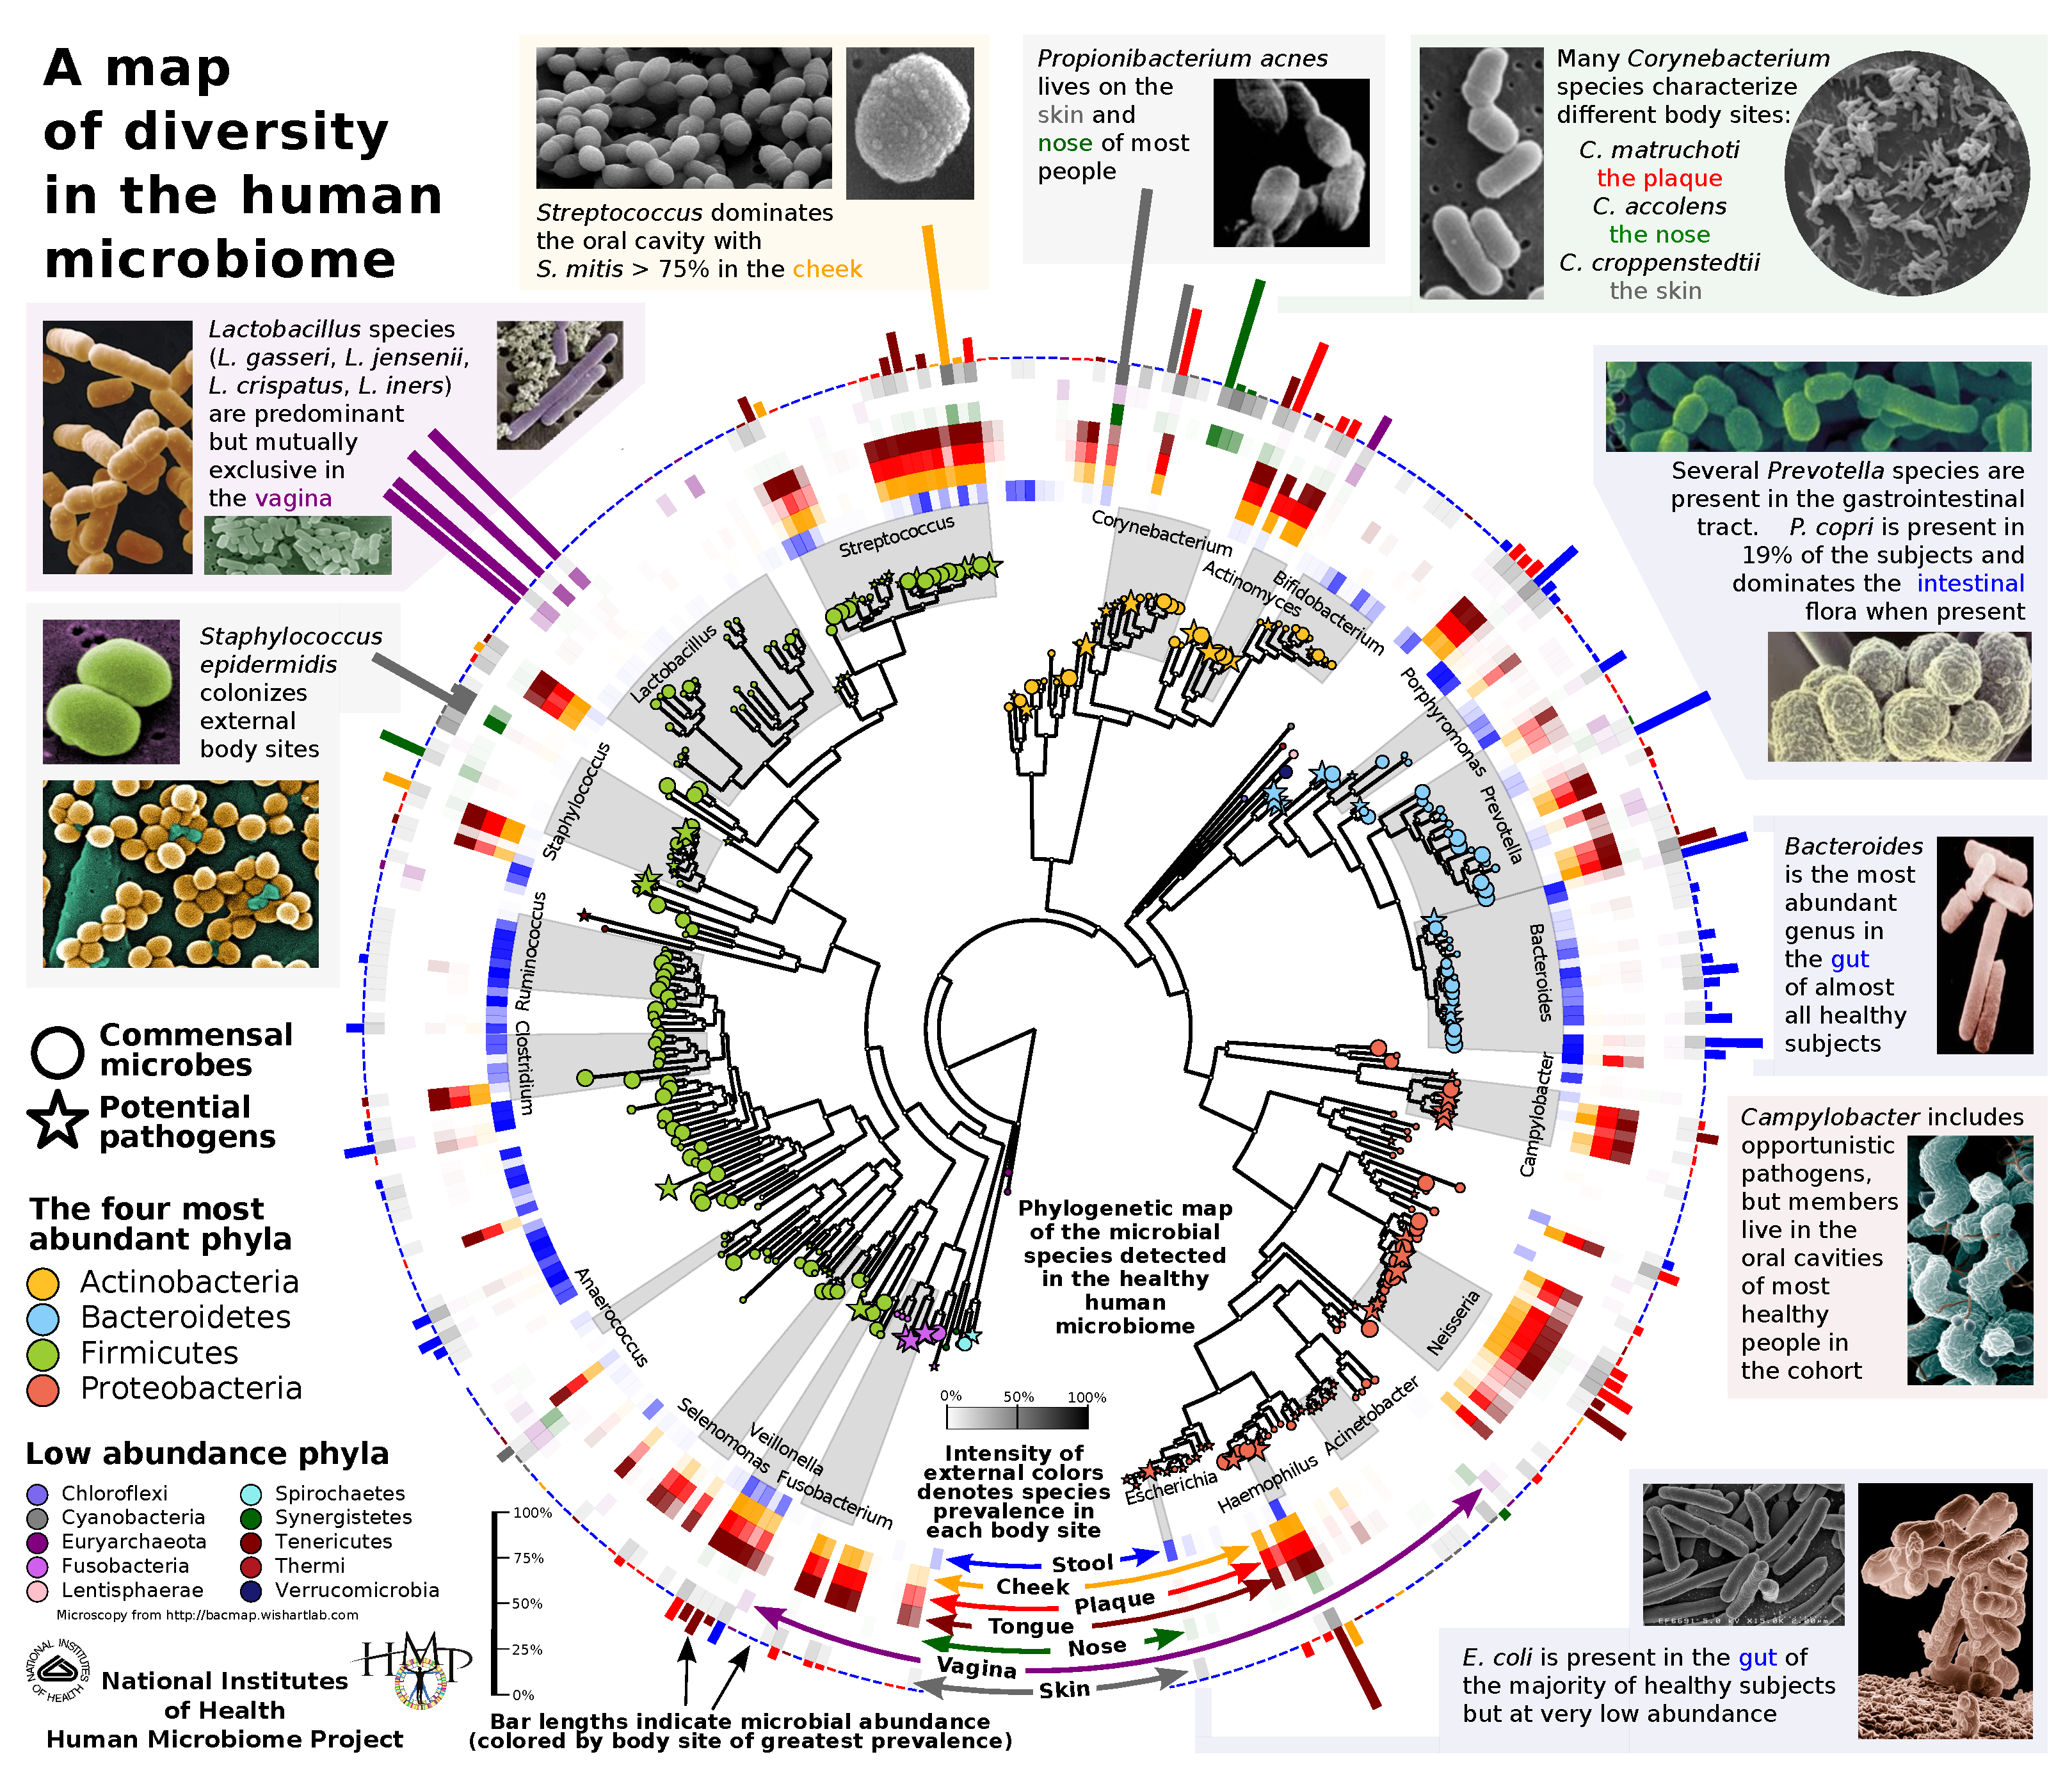
\includegraphics[width=750px,height=580px]{images/humanDiversity} \end{center}

???

\begin{itemize}
\item
  .n{[}Vediamo ora \textbf{dove} sono distribuiti i batteri{]}
\item
  .n{[}Partiamo dalla parte più interna della figura, dall'albero
  filigenetico{]}
\end{itemize}

\begin{center}\includegraphics[width=800px,height=520px]{images/KhoPaperT3-1} \end{center}

\begin{center}\includegraphics[width=900px,height=530px]{images/KhoPaperT3-3} \end{center}

layout: true class: clear

\begin{center}\rule{0.5\linewidth}{0.5pt}\end{center}

\begin{center}\includegraphics[width=630px]{images/PlantmicroPublications} \end{center}

class: inverse, middle, center

\begin{center}\rule{0.5\linewidth}{0.5pt}\end{center}

\begin{center}\rule{0.5\linewidth}{0.5pt}\end{center}

\hypertarget{glossario}{%
\subsection{Glossario}\label{glossario}}

\begin{itemize}
\tightlist
\item
  .font80{[}\textbf{Rhizosphere}: The region of soil in the vicinity of
  plant roots that is influenced by plant-derived nutrients and oxygen
  availability; it is not a region of definable size or shape, but
  instead consists of a gradient in chemical, biological and physical
  properties that change both radially and longitudinally along the
  root.{]}
\end{itemize}

--

\begin{itemize}
\tightlist
\item
  .font80{[}\textbf{Phyllosphere}: All the aboveground organs of plants,
  including the leaf, flower, stem and fruit.{]}
\end{itemize}

--

\begin{itemize}
\tightlist
\item
  .font80{[}\textbf{Endophytes}: The microorganisms residing within
  plant tissues (the endosphere), such as leaves, roots or stems.{]}
\end{itemize}

--

\begin{itemize}
\tightlist
\item
  .font80{[}\textbf{Bulk soil}: is soil outside the rhizosphere. Bulk
  soil is not penetrated by plant roots{]}
\end{itemize}

\begin{center}\rule{0.5\linewidth}{0.5pt}\end{center}

layout: true \# Composizione del microbiota

\begin{center}\rule{0.5\linewidth}{0.5pt}\end{center}

.center{[} .h20{[} \textbf{Spatial plant microbiota}\\
.font50{[}(Singh, Raina, Kumar, et al., 2019){]}{]}

\begin{center}\includegraphics[width=470px,height=470px]{images/PlantMicrobiomeComposition} \end{center}

{]}

\begin{center}\rule{0.5\linewidth}{0.5pt}\end{center}

.center{[} .h20{[} \textbf{Temporal plant microbiota}\\
.font50{[}(Sapkota, Jørgensen, and Nicolaisen, 2017){]}{]}

\begin{center}\includegraphics[width=530px,height=470px]{images/plantMicrobiotaTemporal} \end{center}

{]}

???

.n30{[}

\begin{itemize}
\item
  La composzione del microbiota vegetale è, come quella umana,
  dipendente dalla fase evolutiva della pianta e dal comparto che si
  sceglie di studiare.
\item
  La figura sulla sinistra dello schermo cerca di schematizzare i
  recenti studi fatti sul microbiota delle piante
\end{itemize}

{]}

\begin{center}\rule{0.5\linewidth}{0.5pt}\end{center}

\textbf{Microbiota reservoir}

.pull-left{[} - .n{[}Although the assemblies of root-associated bacteria
and fungi differ substantially from the above-ground communities, both
represent a \textbf{subset of the microbiota derived from soil
communities} and enriched in different plant-associated niches{]}

\begin{itemize}
\tightlist
\item
  .n{[}This suggests that \textbf{soil functions as a common reservoir}
  for both belowground and aboveground plant microbiota{]} {]}
\end{itemize}

.pull-rigth{[}

.h20{[}

\begin{center}\includegraphics[width=450px,height=450px]{images/reservoir} \end{center}

.right{[}.font50{[}(Agnello, Morelli, and Del Panno, 2020){]}{]} {]} {]}

???

.n30{[} - Un'importante considerazione da fare è che sebbene le comunità
batteriche e fungine che sono associate alla piante siano molto diverse
tra la parte ipogea e la parte epigea della pianta, entrambe
rappresentano un sottogruppo del microbiota derivato dalle comunità del
suolo

\begin{itemize}
\tightlist
\item
  Possiamo quindi dire che il suolo funziona come riserva comune per il
  microbiota della pianta epigeo e ipogeo {]}
\end{itemize}

\begin{center}\rule{0.5\linewidth}{0.5pt}\end{center}

.pull-left{[}

\begin{center}\includegraphics[width=350px]{images/bacterialDiv} \end{center}

\begin{center}\includegraphics[width=350px]{images/fungalDiv} \end{center}

{]}

.pull-right{[}

\begin{itemize}
\tightlist
\item
  .n{[}There are clear differences among the microbial communities in
  different plant compartments, which indicates that the \textbf{plant
  compartment is a major selective force} that shapes the composition of
  plant-associated microbiota{]}
\end{itemize}

{]}

???

\begin{itemize}
\item
  .n{[}\textbf{Shannon diversity index}: combina ricchezza e
  diversità{]}
\item
  .n{[}Misura sia il numero delle specie presenti e la differenza tra
  l'abbondanza delle diverse specie.{]}
\item
  .n{[}Un valore grande significa che sono presenti molte specie con
  un'abbondanza simile. Il range del valore varia da 1 (una specie
  dominante) fino al numero totale di tutte le species (nel caso che
  tutte le specie abbiano la stessa abbondanza){]}
\end{itemize}

class: inverse, middle, center

\begin{center}\rule{0.5\linewidth}{0.5pt}\end{center}

\begin{center}\rule{0.5\linewidth}{0.5pt}\end{center}

.center{[}\textbf{There are two major approaches to assess the
microbiota composition}{]}

.h20{[}

\begin{center}\includegraphics[width=520px]{images/microbiotaCompositionTecniques} \end{center}

.right{[}.font60{[}(Lebeis, 2014){]}{]} {]}

\begin{center}\rule{0.5\linewidth}{0.5pt}\end{center}

.pull-left{[}

\begin{center}\includegraphics[width=520px]{images/microbiotaCompositionTecniques} \end{center}

{]}

.pull-right{[} \textbf{Culture dependent}

\begin{itemize}
\item
  This approach isolates individual microbes
\item
  The community diversity estimate is limited
\end{itemize}

{]}

\end{document}
